%%%%%%%%%%%%%%%%%%%%%%%%%%%%%%%%%%%%%%%
% Wenneker Resume/CV
% LaTeX Template
% Version 1.1 (19/6/2016)
%
% This template has been downloaded from:
% http://www.LaTeXTemplates.com
%
% Original author:
% Frits Wenneker (http://www.howtotex.com) with extensive modifications by 
% Vel (vel@LaTeXTemplates.com)
%
% License:
% CC BY-NC-SA 3.0 (http://creativecommons.org/licenses/by-nc-sa/3.0/
%
%%%%%%%%%%%%%%%%%%%%%%%%%%%%%%%%%%%%%%

%----------------------------------------------------------------------------------------
%	PACKAGES AND OTHER DOCUMENT CONFIGURATIONS
%----------------------------------------------------------------------------------------

\documentclass[a4paper,10pt]{memoir} % Font and paper size

%%%%%%%%%%%%%%%%%%%%%%%%%%%%%%%%%%%%%%%%%
% Wenneker Resume/CV
% Structure Specification File
% Version 1.1 (19/6/2016)
%
% This file has been downloaded from:
% http://www.LaTeXTemplates.com
%
% Original author:
% Frits Wenneker (http://www.howtotex.com) with extensive modifications by 
% Vel (vel@latextemplates.com)
%
% License:
% CC BY-NC-SA 3.0 (http://creativecommons.org/licenses/by-nc-sa/3.0/)
%
%%%%%%%%%%%%%%%%%%%%%%%%%%%%%%%%%%%%%%%%%

%----------------------------------------------------------------------------------------
%	PACKAGES AND OTHER DOCUMENT CONFIGURATIONS
%----------------------------------------------------------------------------------------

\usepackage{XCharter} % Use the Bitstream Charter font
\usepackage[utf8]{inputenc} % Required for inputting international characters
\usepackage[T1]{fontenc} % Output font encoding for international characters

\usepackage[top=1cm,left=1cm,right=1cm,bottom=1cm]{geometry} % Modify margins

\usepackage{graphicx} % Required for figures

\usepackage{flowfram} % Required for the multi-column layout

\usepackage{url} % URLs

\usepackage[usenames,dvipsnames]{xcolor} % Required for custom colours

\usepackage{tikz} % Required for the horizontal rule

\usepackage{enumitem} % Required for modifying lists
\setlist{noitemsep,nolistsep} % Remove spacing within and around lists

\setlength{\columnsep}{\baselineskip} % Set the spacing between columns

% Define the left frame (sidebar)
\newflowframe{0.2\textwidth}{\textheight}{0pt}{0pt}[left]
\newlength{\LeftMainSep}
\setlength{\LeftMainSep}{0.2\textwidth}
\addtolength{\LeftMainSep}{1\columnsep}
 
% Small static frame for the vertical line
\newstaticframe{1.5pt}{\textheight}{\LeftMainSep}{0pt}
 
% Content of the static frame with the vertical line
\begin{staticcontents}{1}
\hfill
\tikz{\draw[loosely dotted,color=RoyalBlue,line width=1.5pt,yshift=0](0,0) -- (0,\textheight);}
\hfill\mbox{}
\end{staticcontents}
 
% Define the right frame (main body)
\addtolength{\LeftMainSep}{1.5pt}
\addtolength{\LeftMainSep}{1\columnsep}
\newflowframe{0.7\textwidth}{\textheight}{\LeftMainSep}{0pt}[main01]

\pagestyle{empty} % Disable all page numbering

\setlength{\parindent}{0pt} % Stop paragraph indentation

%----------------------------------------------------------------------------------------
%	NEW COMMANDS
%----------------------------------------------------------------------------------------

\newcommand{\userinformation}[1]{\renewcommand{\userinformation}{#1}} % Define a new command for the CV user's information that goes into the left column

\newcommand{\cvheading}[1]{{\Huge\bfseries\color{RoyalBlue} #1} \par\vspace{.6\baselineskip}} % New command for the CV heading
\newcommand{\cvsubheading}[1]{{\Large\bfseries #1} \bigbreak} % New command for the CV subheading

\newcommand{\Sep}{\vspace{1em}} % New command for the spacing between headings
\newcommand{\SmallSep}{\vspace{0.5em}} % New command for the spacing within headings

\newcommand{\aboutme}[2]{ % New command for the about me section
\textbf{\color{RoyalBlue} #1}~~#2\par\Sep
}
	
\newcommand{\CVSection}[1]{ % New command for the headings within sections
{\Large\textbf{#1}}\par
\SmallSep % Used for spacing
}

\newcommand{\CVItem}[2]{ % New command for the item descriptions
\textbf{\color{RoyalBlue} #1}\par
#2
\SmallSep % Used for spacing
}

\newcommand{\bluebullet}{\textcolor{RoyalBlue}{$\circ$}~~} % New command for the blue bullets
 % Include the file specifying document layout and packages

%----------------------------------------------------------------------------------------
%	NAME AND CONTACT INFORMATION 
%----------------------------------------------------------------------------------------

\userinformation{ % Set the content that goes into the sidebar of each page
\begin{flushright}
% Comment out this figure block if you don't want a photo
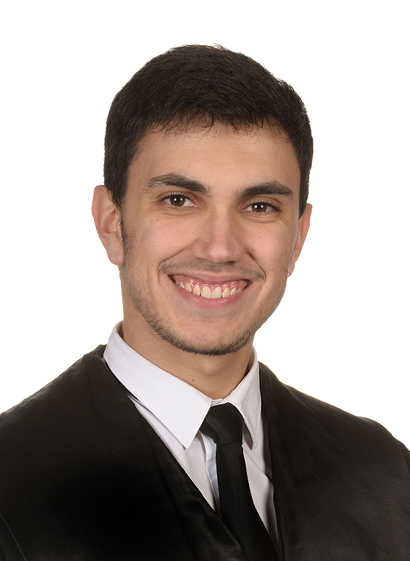
\includegraphics[width=1.0\columnwidth]{photo.jpg}\\[\baselineskip] % Your photo
\small % Smaller font size
Albert Suarez \\ % Your name
\url{alsumo95@gmail.com} \\ % Your email address
\url{www.github.com/AlbertSuarez} \\ % Your URL
(+34) 644 577 607 \\ % Your phone number
\Sep % Some whitespace
\vfill % Whitespace under this block to push it up under the photo
\end{flushright}
}

%----------------------------------------------------------------------------------------

\begin{document}

\userinformation % Print your information in the left column

\framebreak % End of the first column

%----------------------------------------------------------------------------------------
%	HEADING
%----------------------------------------------------------------------------------------

\cvheading{Albert Suarez} % Large heading - your name

\cvsubheading{Software Engineer} % Subheading - your occupation/specialization

%----------------------------------------------------------------------------------------
%	ABOUT ME
%----------------------------------------------------------------------------------------

\aboutme{About Me}{I'm a Software Engineer graduated in Universitat Politecnica de Catalunya, BarcelonaTech. I consider myself a hardworker and focused person. I like talking with new people that can provide me with new knowledge and board in my own ideas. I also love sports, music and travelling.}

%----------------------------------------------------------------------------------------
%	EDUCATION
%----------------------------------------------------------------------------------------

\CVSection{Education}

%------------------------------------------------

\CVItem{2013 - 2017, Universitat Politecnica de Catalunya - BarcelonaTech}{Bachelor degree in Software Engineering}

%------------------------------------------------

\Sep % Extra whitespace after the end of a major section

%----------------------------------------------------------------------------------------
%	EXPERIENCE
%----------------------------------------------------------------------------------------

\CVSection{Experience}

%------------------------------------------------

\CVItem{June 2016 - present, \textit{Co Director \& Organiser}, HackUPC}{
This group of people called Hack UPC organizes the first student Hackathon in Spain. In order to organize this event, I am working as a co-director in the organization. I am responsible for managing and coordinating a team of 25 organizers, event design, logistics, volunteers, sponsorship and marketing.}

%------------------------------------------------

\CVItem{September 2016 - July 2017, \textit{Software Developer Intern}, UPCnet}{While working for UPCNet, I am in a big work team. In order to carry out my duties, I have to use programming languages like Java, frameworks like Spring or Hibernate, working with WebServices (SOAP, WSDL...) and IDEAs like Spring Tool Suite or IntelliJ and designing websites with HTML, CSS, JavaScript, Bootstrap, Sass, Less, JQuery and Handlebars. In conclusion, I am currently training to achieve the objective of become to Full Stack Java Developer.}

%------------------------------------------------

\CVItem{February 2016 - June 2017, \textit{Teacher}, Ases Academy}{Professor of university students, near BarcelonaTech. Currently, I am teaching two subjects: Data Structures and Algorithms and Operative Systems. I teach to student groups with 20-30 people. I really like teach and share my knowledge with university mates.}

%------------------------------------------------

\Sep % Extra whitespace after the end of a major section

%----------------------------------------------------------------------------------------
%	LANGUAGES
%----------------------------------------------------------------------------------------

\CVSection{Languages}

%------------------------------------------------

{\begin{tabular}{p{0.3\textwidth} p{0.3\textwidth}}
\bluebullet Spanish - Native 				&  \bluebullet Catalan - Native\\
\bluebullet English - Academic IELTS 6 (B2)	&  \bluebullet French - Elementary proficiency\\
\end{tabular}}
%------------------------------------------------

\Sep % Extra whitespace after the end of a major section

%----------------------------------------------------------------------------------------
%	PROJECTS
%----------------------------------------------------------------------------------------

\CVSection{Projects}

%------------------------------------------------

\CVItem{Wisebite}{An intelligent platform to manage your restaurant. It allows to create your commands, make a detailed study of your business, join your establishment in a customers network and, briefly, make your restaurant intelligent.}

%------------------------------------------------

\CVItem{Cityfind}{Web application developed in a hackathon situated in Copenhagen called CopenHacks, which is organized by Microsoft. CityFind is a funny way to discover the city. Just enter into the platform, register a room and share the room number with your friends. Once you are ready, the creator of the room will start the game. Each of the participants will get an SMS to their mobile phone with a timer and a thing. They will have this time to take a photo with this thing. The photo will be validated using MS cognitive services. If the photo is validated, the participant will earn point. When ending the game, the participant with more points wins.}

%------------------------------------------------

\CVItem{Blunch}{From the tendency of collaborative economy Blunch arises, a platform which allows its community to sell dishes or participate in a “Collaborative menu” by exchanging dishes provided by each participant. Blunch provides a useful, intuitive and secure way to meet new people, reduce the waste of food and earn some money on the way.}

%------------------------------------------------

\Sep % Extra whitespace after the end of a major section

%----------------------------------------------------------------------------------------
%	SKILLS
%----------------------------------------------------------------------------------------

\CVSection{Featured Skills \& Endorsements}

{\begin{tabular}{p{0.2\textwidth} p{0.2\textwidth} p{0.2\textwidth}}
\bluebullet Java 		&  \bluebullet Android		& \bluebullet C++\\
\bluebullet Python 		&  \bluebullet Linux		& \bluebullet SQL\\
\bluebullet Git 		&  \bluebullet Agile		& \bluebullet Web development\\
\bluebullet Maven 		&  \bluebullet Teaching		& \bluebullet Leadership\\
\end{tabular}}

\end{document}
